\documentclass[conference]{IEEEtran}
\usepackage[english,portuguese]{babel}
\usepackage{blindtext, graphicx}
\usepackage{listings}
\lstset{
  language=C++,
  numbers=left,
  breaklines=true,
  xleftmargin=4em,
  resetmargins=true,
  basicstyle=\footnotesize,
  numberstyle=\footnotesize,
}
\usepackage{graphicx}
\usepackage[font=small]{caption}
\usepackage[utf8]{inputenc}
\usepackage{array}
\usepackage{mathtools}
\usepackage{float}

\selectlanguage{portuguese}

\newenvironment{conditions}
  {\par\vspace{\abovedisplayskip}\noindent\begin{tabular}{>{$}l<{$} @{${}={}$} l}}
  {\end{tabular}\par\vspace{\belowdisplayskip}}

\title{Diagnóstico da doença de Alzheimer usando imagens de ressonância magnética por rede neural convolucional}

\author{
  \IEEEauthorblockN{Marlon Valmórbida Cendron}
  \IEEEauthorblockA{
    \textit{Ciência da Computação, IFC}\\
    Videira, Brasil\\
    marlonvcendron@gmail.com}
}

\begin{document}

\maketitle

\begin{abstract}
  A doença de Alzheimer (DA) é uma doença neurodegenerativa que vem aumentando conforme a expectativa de vida aumenta e é a principal causa de demência no mundo. Quanto antes detectada e tratada a doença, menores serão os problemas causados ao paciente. Usando imagens de ressonância magnética (IRM) é possível diagnosticar a doença. Um profissional pode diagnosticar um paciente com sensibilidade entre 70,9\% e 87,3\% e especificidade entre 44,3\% e 70,8\%. A utilização de um método automático de diagnóstico precoce da DA por meio de um algoritmo de aprendizado de máquina tem o potencial de ter maior precisão que especialistas da área. Neste trabalho foi construída uma rede neural convolucional com a intenção de diagnosticar fatias de IRM com a DA. Por mais que essa tarefa seja possível, nesse trabalho a falta de dados fez com que a rede neural acabasse não aprendendo. 
\end{abstract}
  
\global\long\def\IEEEkeywordsname{Palavras-chave}

\begin{IEEEkeywords}
  Alzheimer, diagnóstico, ressonância magnética, aprendizado de máquina, rede neural convolucional
\end{IEEEkeywords}

\selectlanguage{english}
\begin{abstract}
  Alzheimer's disease (AD) is a neurodegenerative disease that has been increasing as life expectancy increases and is the leading cause of dementia in the world. The earlier the disease is detected and treated, the lesser the problems caused to the patient. Using magnetic resonance imaging (MRI) it is possible to diagnose the disease. A professional can diagnose a patient with sensitivity between 70.9\% and 87.3\% and specificity between 44.3\% and 70.8\%. The use of an automatic method of early diagnosis of AD through a machine learning algorithm has the potential to be more accurate than specialists in the field. In this work, a convolutional neural network was built with the intention of diagnosing MRI slices with AD. As much as this task is possible, in this work the lack of data meant that the neural network ended up not learning.
\end{abstract}
  
\global\long\def\IEEEkeywordsname{Keywords}

\begin{IEEEkeywords}
  Alzheimer, diagnosis, magnetic resonance, machine learning, convolutional neural network
\end{IEEEkeywords}

\selectlanguage{portuguese}


\section{Introdução}

O cérebro é o órgão central na cognição humana. Com o recente aumento da expectativa de vida na históra da humanidade, viu-se um aumento considerável nos casos de doença de Alzheimer (DA), uma doença degenerativa do cérebro que causa a morte de neurônios, caracterizada pela perda de memória, redução da capacidade cognitiva entre outros. A doença é mais comum a partir da idade de 60 anos, mas pode acontecer precocemente a partir dos 40 anos em casos de recorrência familiar \cite{alzheimer}. Quanto antes detectada e tratada a doença, menores serão os problemas causados ao paciente.

Usando imagens de ressonância magnética (IRM) do cérebro em um paciente em estado avançado de DA, como na figura \ref{fig:alzheimer}, é clara a diferença com um cérebro saudável, mas nos estados iniciais, essa diferença não é tão clara. Um profissional pode diagnosticar um paciente com sensibilidade entre 70,9\% e 87,3\% e especificidade entre 44,3\% e 70,8\%. A utilização de um método automático de diagnóstico precoce da DA por meio de um algoritmo de aprendizado de máquina tem o potencial de ter maior precisão que especialistas da área, como em \cite{alkhuzaie} onde foi maior que 97\%.

O tipo de algoritmo de aprendizado de máquina mais utilizado para classificação e regressão a partir de imagens de entrada são as redes neurais convolucionais (RNC). Esse tipo de rede neural tem um neurônio artificial para cada pixel da imagem de entrada e são aplicadas diversas convoluções para processar a imagem e adquirir um resultado. Quais tipos de convolução devem ser aplicadas são aprendidas durante a fase de treinamento da RNC, que, no caso da classificação, consiste em processar as imagens inicialmente com convoluções aleatórias, verificar a classificação adquirida (Diagnosticado com ou sem DA) e aplicar os algoritmos de retropropagação e descida do gradiente para ajustar os valores das convoluções para se ter um resultado mais próximo do resultado esperado, que de início será apenas aleatório, pois a rede ainda não aprendeu.

Neste trabalho é apresentada uma rede neural convolucional para diagnosticar a DA a partir de uma fatia de um IRM, sem utilizar a imagem volumétrica inteira. A rede não se otimizar para gerar resultados satisfatórios.

\section{Fundamentação teórica}

\subsection{Doença de Alzheimer}

A doença de Alzheimer (DA) é uma doença neurodegenerativa que começa lentamente e piora gradativamente. O primeiro sintoma mais comum a aparecer é a perda de memória, que pode ser confundida com o esquecimento normal do envelhecimento. A perda de memória é seguida por dificuldades de linguagem, como a dificuldade de encontrar a palavra certa para descrever algo, e dificuldades de raciocínio, como a dificuldade de resolver problemas matemáticos. A perda de memória e dificuldades de raciocínio podem levar a uma perda de habilidades motoras, como a dificuldade de escrever ou de se vestir.

Atualmente, não há nenhum modo de parar ou reverter a DA, mas um diagnóstico precoce pode ajudar a remediar os sintomas. E, no futuro, é provável que uma possível cura descoberta seja mais eficaz quando aplicada no início do desenvolvimento da doença.

\begin{figure}[H]
\centering
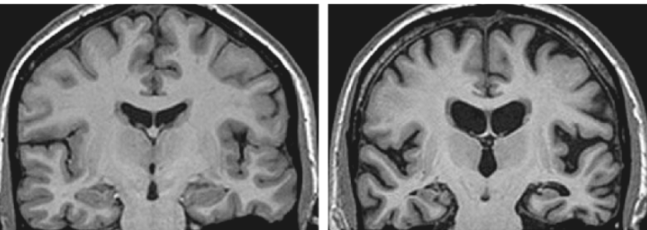
\includegraphics[width=8cm]{img/alzheimer.png}
\caption{Cérebro saudável (esquerda) e com DA (direita)}
\label{fig:alzheimer}
\end{figure}

\subsection{Redes Neurais Convolucionais}

Redes neurais convolucionais (RNC) tomam como inspiração algumas redes neurais do córtex visual, onde conjuntos de neurônios trabalham juntos para detectar padrões. No início do processamento visual do cérebro humano, nas primeiras camadas existem neurônios que detectam padrões como linhas em determinadas orientações, enquanto que nas camadas mais profundas, usando o processamento desses padrões mais simples, os neurônios detectam padrões mais complexos, como círculo e figuras geométricas, e mais fundo ainda, as camadas podem processar objetos ou faces humanas.

Em RNCs, as convoluções são matrizes que são aplicadas sobre a imagem de entrada para detectar padrões. As convoluções são aplicadas sobre a imagem de entrada e o resultado é uma nova imagem, que é então aplicada a outra convolução, e assim por diante. A figura \ref{fig:conv} mostra um exemplo de convolução que destaca bordas.


\begin{figure}[H]
\centering
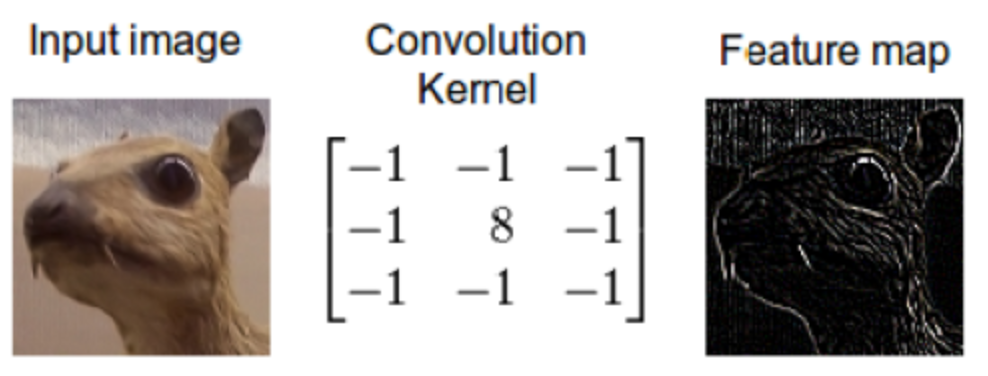
\includegraphics[width=8cm]{img/conv.png}
\caption{Exemplo de convolução que destaca bordas}
\label{fig:conv}
\end{figure}

Através da retropropagação e a descida do gradiente, a RNC é capaz de aprender quais convoluções devem ser aplicadas para obter um resultado mais próximo do resultado esperado.

Ao final das camadas de convoluções, são utilizadas camadas feedforward de uma rede neural convencional, que são capazes de classificar os resultados das convoluções.

Também é comum utilizar camadas de Max Pooling após uma camada de convolução. O Max Pooling funciona quase como um redutor de dimensionalidade: ele é capaz de reduzir a quantidade de dados de entrada, mas mantendo as características mais importantes da imagem. A figura \ref{fig:pool} mostra um exemplo de Max Pooling.

\begin{figure}[H]
\centering
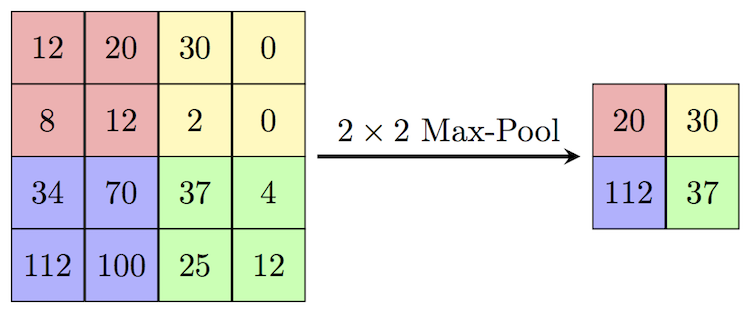
\includegraphics[width=8cm]{img/pool.png}
\caption{Exemplo de Max Pooling}
\label{fig:pool}
\end{figure}

\section{Métodos}

\subsection{Dados}

Foram utizados os dados da Alzheimer's Disease Neuroimaging Initiative, ou Iniciativa de Neuroimagem da Doença de Alzheimer, em tradução livre. O total de dados utilizados foi de 270 IRM, onde 98 eram de pacientes com DA e 172 do grupo de controle. Os dados foram divididos em 2 conjuntos: treinamento, correspondente a \textthreequarters ~do total dos dados, e teste, o \textonequarter~restante. O conjunto de treinamento foi utilizado para treinar a rede neural e o conjunto de teste foi utilizado para verificar a precisão da rede neural.

\begin{figure*}[ht!]
\centering
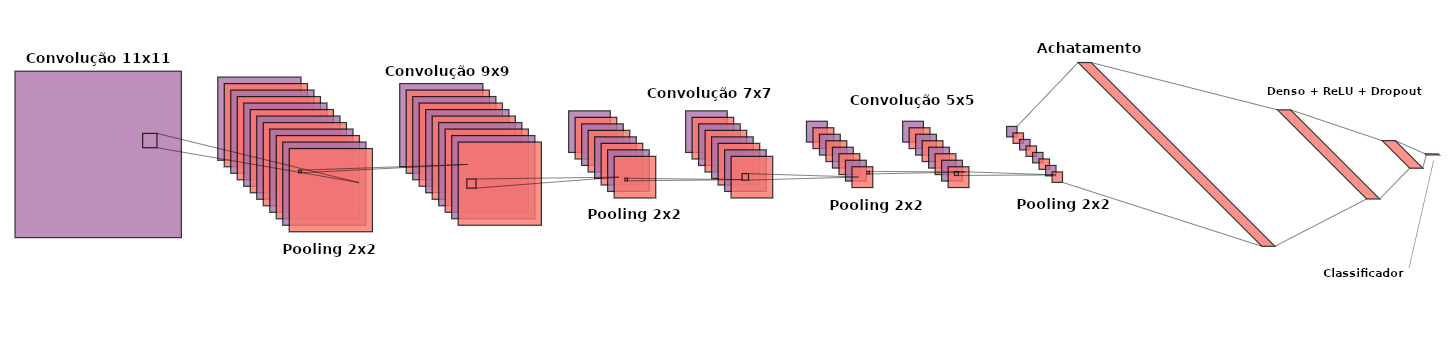
\includegraphics[width=16cm]{img/architecture.png}
\caption{Arquitetura da RNC}
\label{fig:arch}
\end{figure*}

Como a rede foi treinada usando apenas fatias 2D das imagens volumétricas de IRM, 24 fatias da IRM foram utilizadas.

As imagens foram pré-processadas para que a rede neural pudesse aprender melhor. O pré-processamento consistiu em: normalização espacial, extração do crânio e pescoço e normalização dos valores entre 0 e 1. A normalização espacial foi feita para que as imagens tivessem o mesmo tamanho e a mesma resolução. A extração do crânio, como vista na figura \ref{fig:bet}, foi feita para que a rede neural não levasse em consideração a região do crânio, que é uma região que não é afetada pela DA, para tal, foi utilizado o algoritmo BET \cite{bet}. A extração do pescoço usou o algoritmo robustfov. A normalização dos valores entre 0 e 1 foi feita para que a rede neural não tivesse problemas com valores muito altos ou muito baixos.

\begin{figure}[H]
\centering
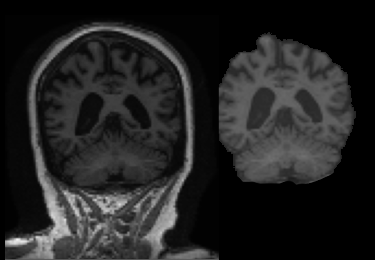
\includegraphics[width=8cm]{img/bet.png}
\caption{Extração do crânio e pescoço}
\label{fig:bet}
\end{figure}

\subsection{Arquitetura da Rede Neural Convolucional}

Foi utilizado Python 3.10 e PyTorch para a implementação da rede neural, e a biblioteca SimpleITK para o pré-processamento das imagens.

A rede, diagramada na figura \ref{fig:arch}, é composta de 4 camadas de convolução com a função de ativação ReLU (Rectified Linear Unit), com camadas de Max Pooling 2x2 entre elas. No final, há uma camada de achatamento para tornar a saída bidimensional da rede em um vetor unidimensional, que é então passado para duas camadas feedforward com 200 e 97 neurônios, respectivamente. A penúltima camada tem 30 neurônios que convergem em um só neurônio final da camada de saída, que é a camada de classificação. A camada de saída tem a função de ativação sigmóide, que retorna um valor entre 0 e 1, que é a probabilidade da imagem ser de um paciente com DA.

\section{Resultados}

Conforme é possível verificar na figura \ref{fig:loss}, o erro ficou oscilando e não diminuiu, ou seja: a rede não foi capaz de aprender. Isso pode ter acontecido por vários motivos, como: a quantidade de dados, a quantidade de fatias utilizadas, a quantidade de épocas de treinamento e o fato de ter mais exemplos do grupo de controle do que com DA. 

\begin{figure}[H]
\centering
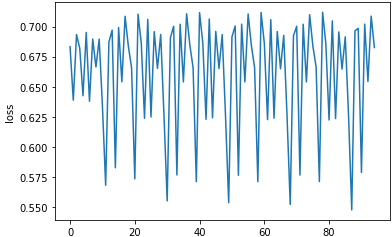
\includegraphics[width=8cm]{img/loss.png}
\caption{Erro durante o treinamento}
\label{fig:loss}
\end{figure}

\section{Conclusão}

Por mais que a normalização dos dados tenha sido bem feita, com uma pequena quantidade de dados e usando apenas fatias em 2D de IRM não foi possível treinar uma RNC para diagnosticar a DA com precisão. O fato de ter muitos mais exemplos do grupo de controle do que com DA também deve ter afetado o resultado. Para que a rede neural pudesse aprender melhor, seria necessário um conjunto de dados maior e mais balanceado.

\bibliographystyle{plain}  
\bibliography{refs}

\end{document}
